\section{Landing hardware requirements}

\subsection{Vehicle hardware}
The hardware requirements for vehicles to perform landing operations are sufficiently different to standard vehicles to warrant specific consideration. In this work, we propose a vehicle concept with negative buoyancy during operation. This minimises the use of vertical thrusters during landing operations, allowing the vehicle to remain stationary and vibration free whilst landed and saves power. 

The features of the vehicle can be seen in the Fig.~\ref{f:mehul2}. Independent heave, surge, sway and heading control are needed to allow the vehicle to operate at low speeds manoeuvres and hover when necessary. Two horizontal thrusters provide surge and heading control. Two thrusters, inclined at $22.5^\circ$ with the vertical, control sway and heave. The inclined thrusters direct thrust away from the area directly below the vehicle to minimizing the disturbance of sand and sediments during landing. A nylon landing skid distributes the vehicle's weight and provides a stable footing when the vehicle has landed. This also provides enough clearence to protect the sensors on the the vehicle.

\begin{figure}[!ht]
\centering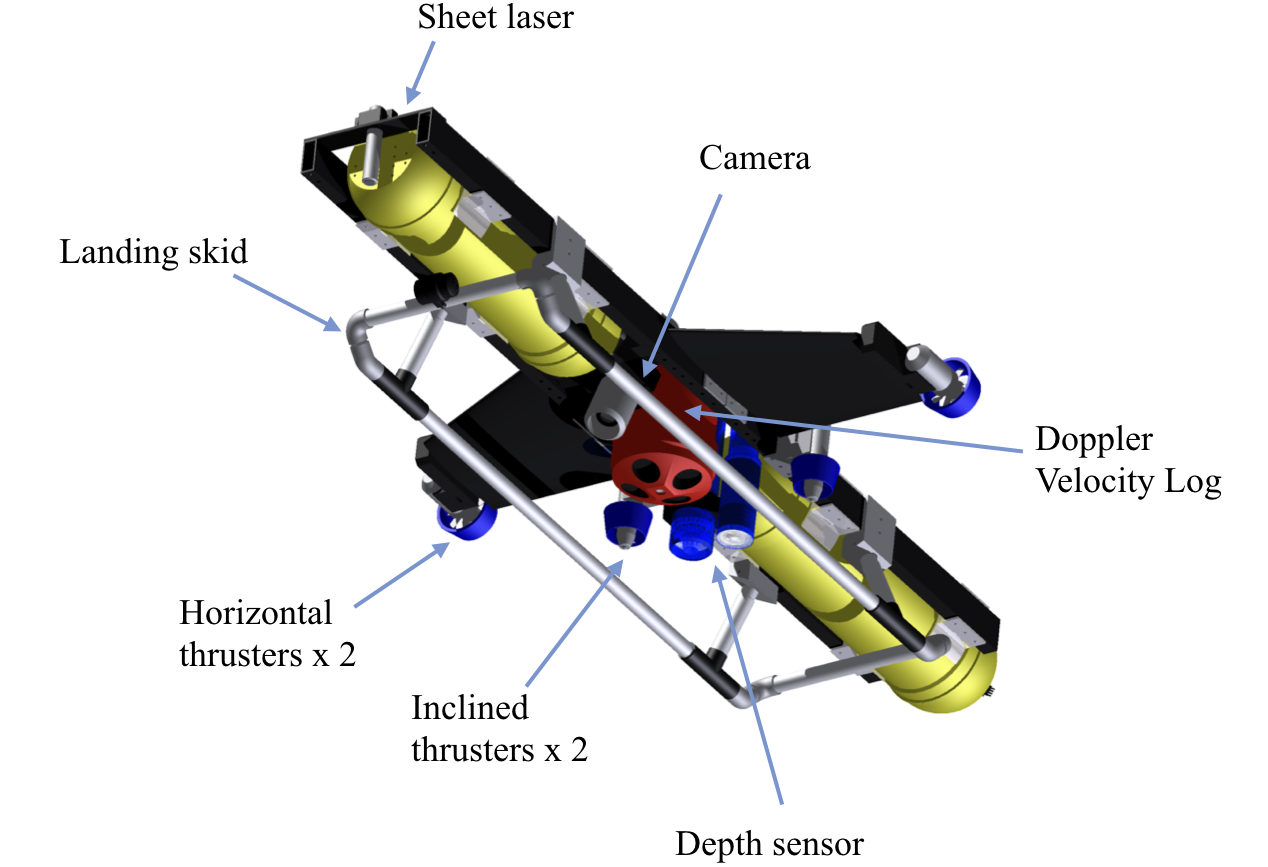
\includegraphics[width=4.5in]{./images/mehul2.png}
\caption{Concept design of a landing vehicle}
\label{f:mehul2}
\end{figure}

The vehicle is designed to be negatively buoyant to allow for landing. Although variable buoyancy engines are available \cite{Zhao2008}, these typically have a capacity of \<1\,L, and the limited change in buoyancy imposes limits on the conditions under which a vehicle can remain securely landed. Here, a hydrodynamic solution is chosen using a fixed wing NACA$651412$ profile to offset the negative buoyancy during forward motion as this approach can compensate for a large change in buoyancy. This profile produces lift at zero angle of attack and so minimising the vehicle's drag. During slow manouvres the vehicle is still able to hover, and ethods such as the two drop weight method can be used for diving and fail-safe surfacing \cite{Thornton2019}. The vehicle has a standard navigation suite, consisting of a 1.2\,MHz Doppler Velocity Log (DVL), raised more than 30\,cm of the bottom of the vehicle to provide bottom lock even when landed, a compass based Attitude Heading Reference System (AHRS), and pressure depth sensor. In addition to standard localisation, the pressure sensor and DVL range can also be used to measure vertical motion during landing and confirm the vehicle remains stationary on the seafloor once landed.

\subsection{High resolution mapping system}
\label{ssec:hres}

A high resolution mapping system using light sectioning is used to generating mm-resolution bathymetry, as illustrated in Fig.~\ref{f:mehul3}~\cite{Bodenmann2016} with associated parameters explained in Table~\ref{t:table0}. The sheet laser projects a line on the seafloor whose projection is captured by an offset camera. By detecting the laser line in the image, it is possible to determine the relative coordinates of each recognised point in the laser line. These can then be used to generate continuous bathymetry measurements in the earth-fixed coordinate system based on the vehicle's pose.

\begin{figure}[!ht]
\centering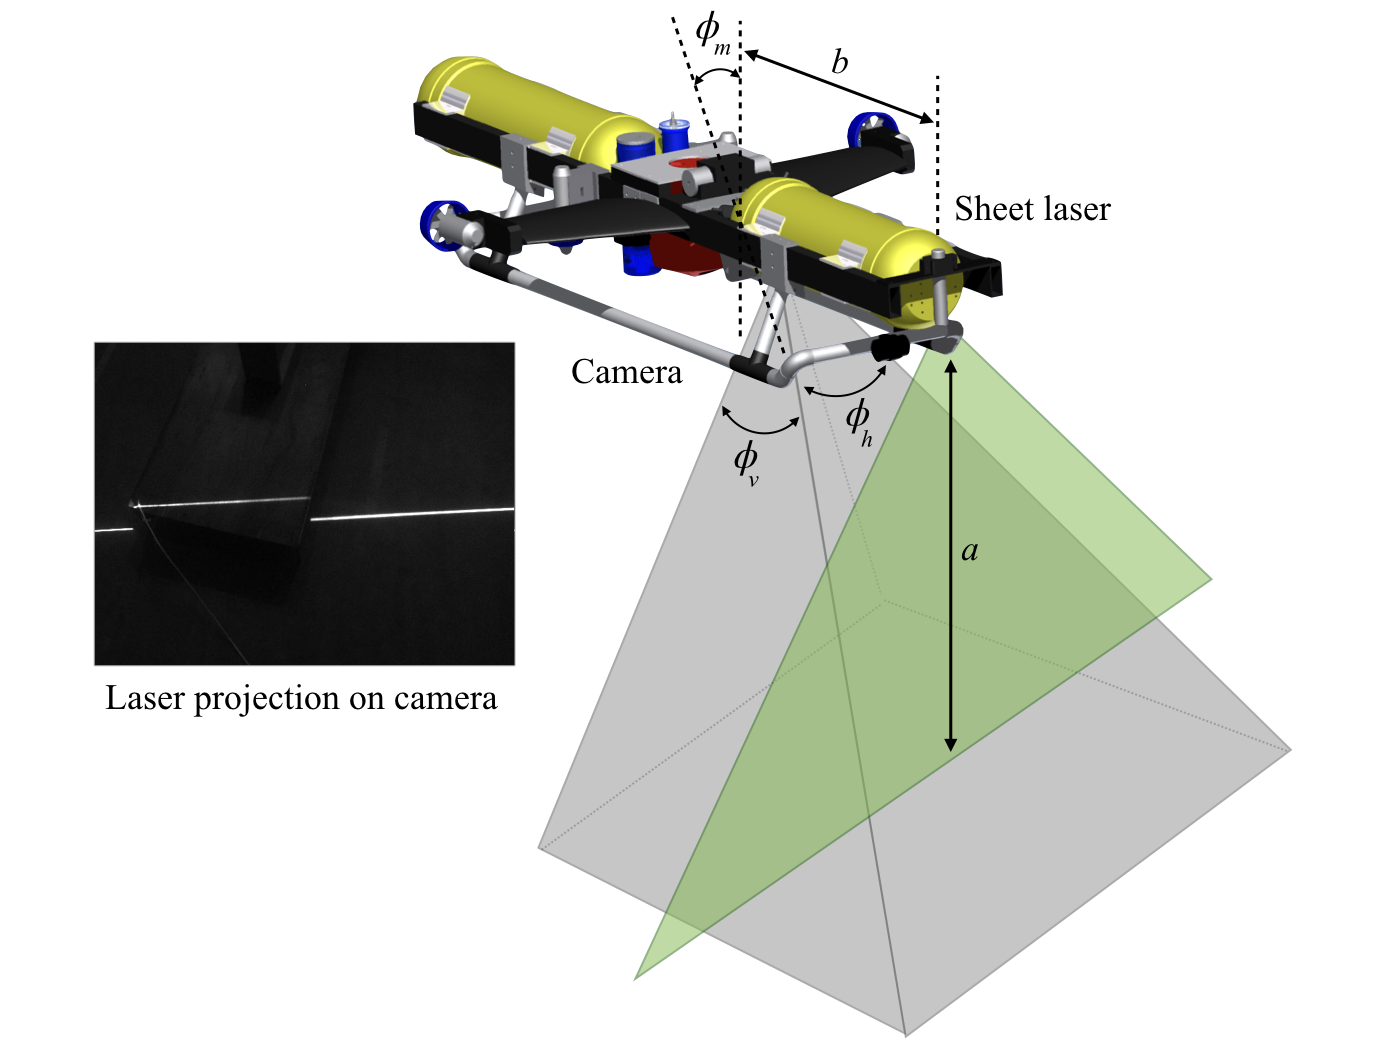
\includegraphics[width=7in]{./images/mehul3.png}
\caption{Setup and working of the high resolution mapping system}
\label{f:mehul3}
\end{figure}

\begin{table}[!ht]
\centering
\caption{Parameters of the mapping system}
\begin{tabular}{  |p{6cm}  p{4cm}| }
\hline
\textbf{Property} & \textbf{Value}\\ \hline 
Mapping altitude & $a$\\
Baseline between camera and laser & $b$\\
Vertical mounting angle of camera & $\phi_m$\\
Horizontal opening angle of camera & $\phi_h$\\
Vertical opening angle of camera & $\phi_v$\\
\hline
\end{tabular}
\label{t:table0}
\end{table}

 